\label{sec:auth-implementation}
\subsubsection{Đăng ký, đăng nhập và dữ liệu công khai}
AuthService chuẩn hóa email bằng trim/lowercase. Đăng ký kiểm email, băm mật khẩu bằng bcrypt với cost 10 rồi tạo User CUSTOMER; đăng nhập dùng compare với hash đã lưu. Sai email hoặc mật khẩu trả cùng thông báo. UsersService dùng select các trường công khai khi tạo/đọc theo id; response không trả passwordHash.

AuthModule cấp access token thời hạn 7 ngày, payload nghiệp vụ gồm sub=id và email; thư viện quản lý trường thời gian. JWT được ký để kiểm chứng, không dùng như dữ liệu bí mật đã mã hóa. Secret lấy ở backend qua cấu hình môi trường. Frontend gửi token qua Authorization: Bearer khi gọi API được bảo vệ.

\subsubsection{Chuỗi kiểm tra JWT, vai trò và chủ đơn}
JwtAuthGuard dùng Passport strategy jwt để kiểm chữ ký và hạn. JwtStrategy.validate đọc lại User theo sub và trả id/email/role vào request.user; vì role lấy từ database ở mỗi lần validate, thay quyền có hiệu lực ở request xác thực tiếp theo mà không đợi token cũ hết hạn. CurrentUser chỉ trích request.user cho controller, không tự xác minh token lần nữa.

Route quầy khai báo UseGuards(JwtAuthGuard, RolesGuard) và Roles(BARISTA). RolesGuard đọc metadata của handler/class, đối chiếu role đã lấy từ database. Với route cá nhân, service còn kiểm userId của Order; có JWT đúng chưa đồng nghĩa được truy cập mọi mã đơn. Việc quyết định trạng thái, credit và version tiếp tục áp dụng sau khi qua lớp quyền.

\subsubsection{Trạng thái đăng nhập ở giao diện}
AuthForm gọi API, lưu accessToken/user vào Zustand persist và điều hướng về trang đang cần hoặc quầy theo role. Tham số next chỉ chấp nhận đường dẫn nội bộ để tránh điều hướng ra website tùy ý. Auth store hiện lưu qua localStorage; logout xóa trạng thái ở trình duyệt. Đây là thao tác kết thúc phiên phía client, không được hiểu là đã thu hồi mọi JWT đã phát hành. Dữ liệu role trên UI phục vụ hiển thị; backend vẫn quyết định quyền thật.

\begin{figure}[htbp]\centering
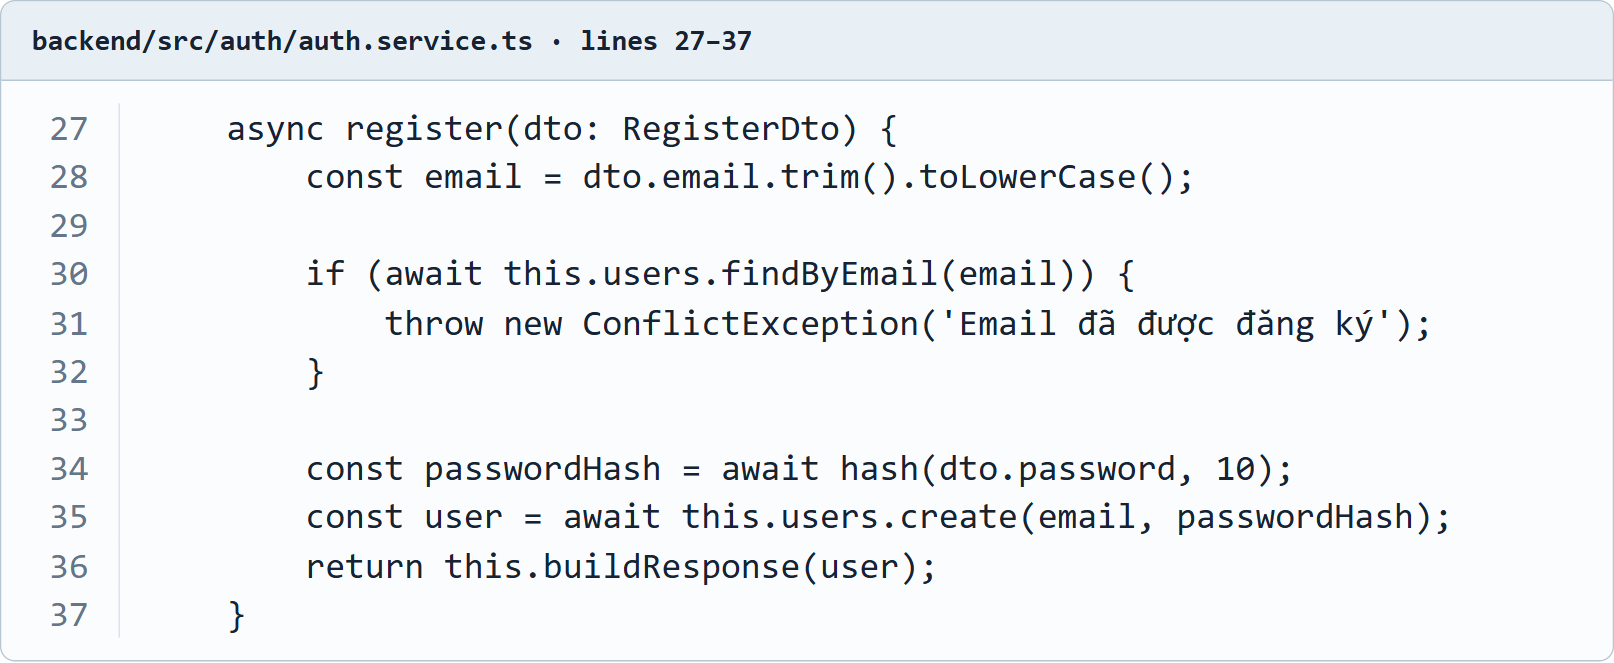
\includegraphics[width=.94\linewidth,height=.23\textheight,keepaspectratio]{assets/auth/code-register.png}
\caption{Đăng ký chuẩn hóa email và lưu hash thay vì mật khẩu gốc}
\vspace{3mm}
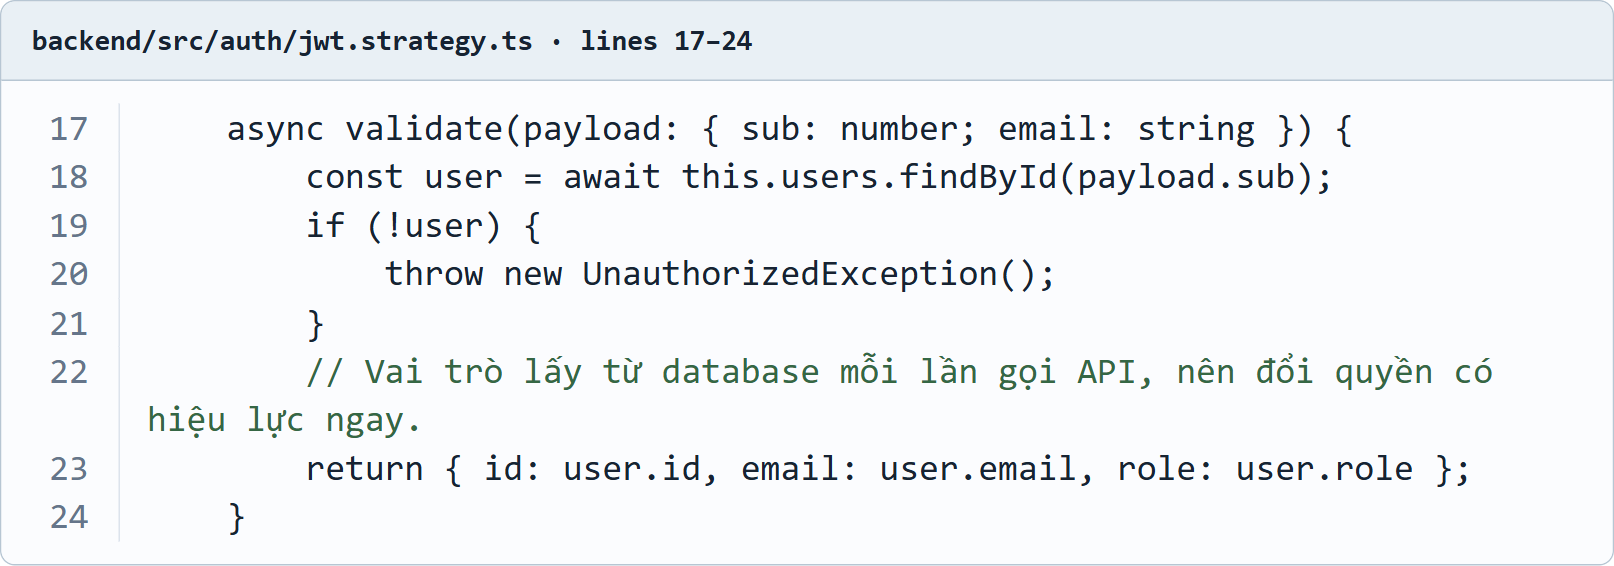
\includegraphics[width=.94\linewidth,height=.23\textheight,keepaspectratio]{assets/auth/code-strategy.png}
\caption{JWT strategy lấy vai trò hiện tại từ User trong database}
\vspace{3mm}
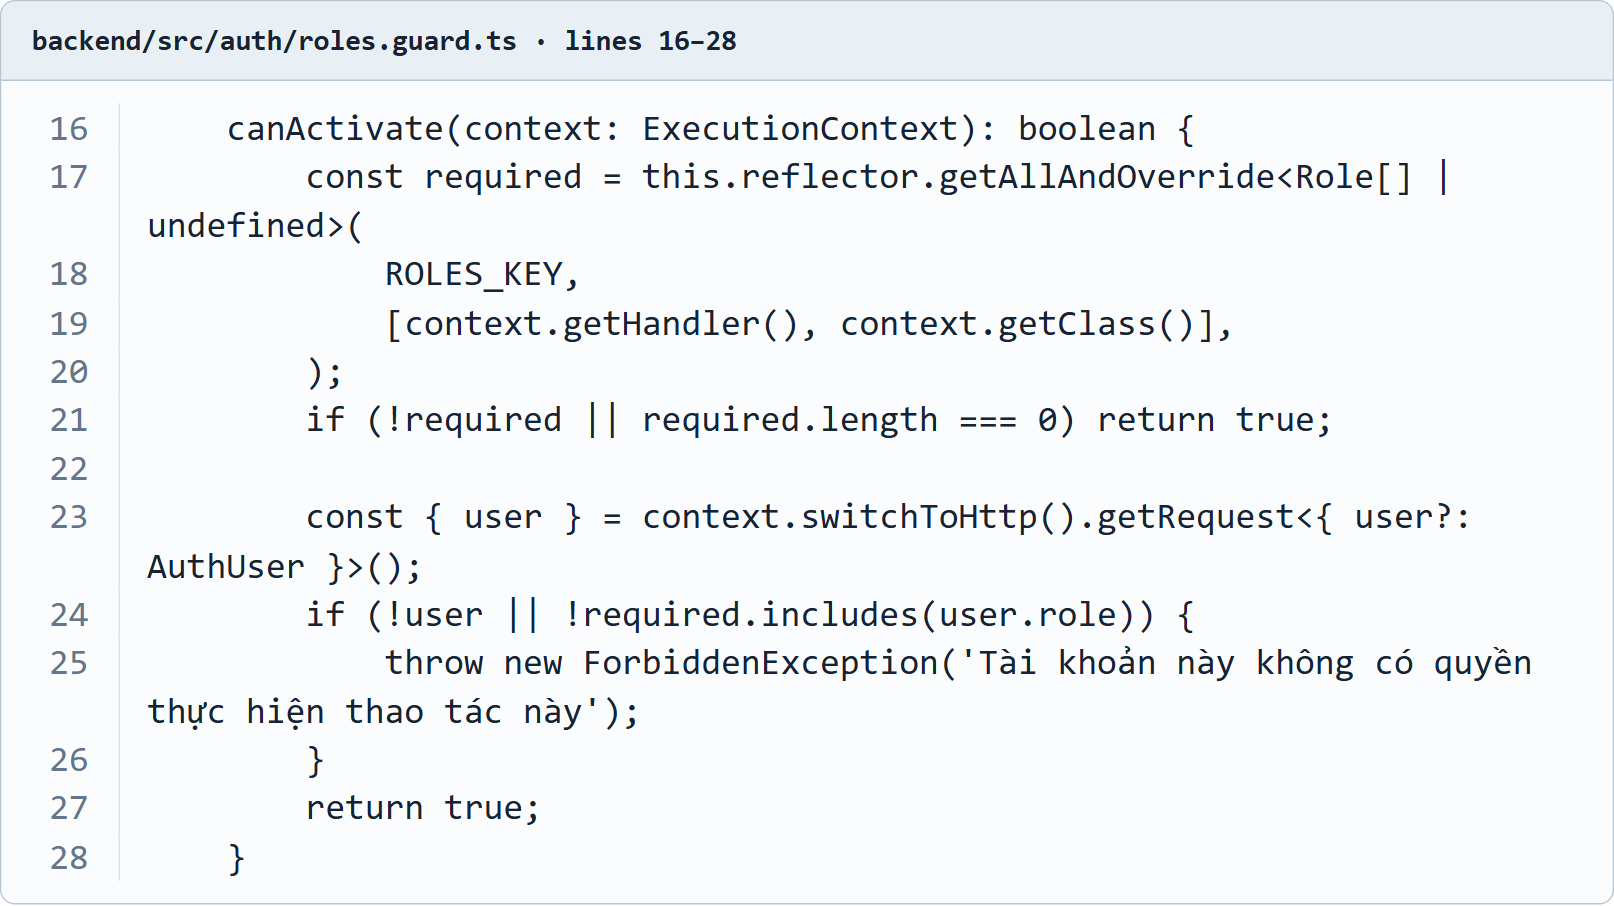
\includegraphics[width=.94\linewidth,height=.25\textheight,keepaspectratio]{assets/auth/code-role.png}
\caption{RolesGuard đối chiếu vai trò với metadata của route}
\end{figure}
